% =============================================================================
%  Examen final - Introduccion a la Computacion Cientifica (Uninorte)
%  Benchmarking de paralelismo de VASP en Granado
%  Rafael Silvera Altamiranda
%
%  Compilar desde reporte/:  pdflatex reporte.tex && pdflatex reporte.tex
%  Las figuras (figuras/) y las tablas (tablas/) las generan los scripts de analisis/.
% =============================================================================
\documentclass[11pt,a4paper]{article}
\usepackage[utf8]{inputenc}
\usepackage[T1]{fontenc}
\usepackage{lmodern}
\usepackage{microtype}
\DisableLigatures[-]{encoding = T1, family = tt*}
\IfFileExists{spanish.ldf}{\usepackage[spanish,es-noshorthands,es-nodecimaldot,es-tabla]{babel}}{%
  \hyphenpenalty=10000 \exhyphenpenalty=10000}
\usepackage[margin=2.1cm,top=1.9cm,bottom=2.1cm]{geometry}
\usepackage{amsmath}
\usepackage{graphicx}
\usepackage{booktabs}
\usepackage{float}
\usepackage[font=small,labelfont=bf,skip=4pt]{caption}
\usepackage{enumitem}
\usepackage{xcolor}
\usepackage{adjustbox}
\usepackage[colorlinks=true,linkcolor=blue!50!black,citecolor=blue!50!black,urlcolor=blue!50!black]{hyperref}
\setlist{itemsep=1pt,topsep=3pt,parsep=0pt}
\setlength{\parskip}{3pt}
\emergencystretch=3em
\tolerance=1500
\newcommand{\eps}{\varepsilon_\mathrm{mach}}
\newcommand{\cod}[1]{\texttt{#1}}

\begin{document}
\renewcommand{\figurename}{Figura}
\renewcommand{\tablename}{Tabla}
\renewcommand{\abstractname}{Resumen}
\renewcommand{\refname}{Referencias}

\begin{center}
{\Large\bfseries Benchmarking de paralelismo de VASP en Granado:\\[2pt]
WSe$_2$ con una vacancia de Se}\\[6pt]
Rafael Silvera Altamiranda \quad·\quad Introducción a la Computación Científica, Universidad del Norte\\
Examen final, Ruta A (VASP) \quad·\quad noviembre de 2026 \quad·\quad repositorio \cod{examen\_silvera/}
\end{center}

\begin{abstract}
\noindent
Se caracterizó el paralelismo de VASP~6.3.0 en un nodo de Granado (2~sockets $\times$ 18 núcleos Xeon Gold~6140)
con un cálculo SCF de WSe$_2$ con una vacancia de Se (23 átomos, 36 k-points; 31.2~min en un núcleo). Con MPI
(paralelismo sobre bandas) la aceleración llega a $S(24)=6.49$ ($E=0.27$); la ley de Amdahl da $f=0.095$,
pero la fracción de Karp--Flatt crece de 0.08 a 0.12, señal de un sobrecosto que aumenta con $p$. Con OpenMP
(un proceso, binario sin \cod{fftlib}) la aceleración máxima es 1.39 con 4 hilos y con 24 hilos el cálculo es
más lento que en serie. En escalamiento débil (KPAR $=p$, 3 k-points por proceso) $E_w(24)=0.50$: toda la
pérdida está en el eigensolver, sin comunicación, es decir, en la contención por recursos compartidos del nodo;
además la memoria por proceso crece con el número total de k-points y la total pasaría el límite de la QOS en
$p\approx29$. Con 24 núcleos el óptimo híbrido es 24 procesos MPI $\times$ 1 hilo; $12\times2$ es 3\,\% más
lento con 40\,\% menos memoria. Las energías convergidas con $p=1$ a 24 difieren en $\le2.6\times10^{-8}$~eV
($7\times10^{5}\,\eps|E|$), 40 veces menos que el criterio de convergencia. ENCUT~$=400$~eV es el punto de
rendimientos decrecientes (0.33~meV/átomo). Recomendación: MPI puro con KPAR~$=12$ en 12 núcleos, 3.9~min y
0.79~h-núcleo por cálculo, más rápido y 2.4 veces más barato que 24 núcleos sin KPAR. Consumo total:
148.5 de 250 h-núcleo.
\end{abstract}

% =============================================================================
\section{Sistema, caso base y metodología}

\paragraph{Sistema (Tarea 0).} 2H-WSe$_2$ en volumen, supercelda $2\times2\times1$ con una vacancia de Se
(el defecto de mi tesis), con la geometría experimental sin relajar ($a=3.282$~Å, $c=12.96$~Å) y un SCF
estático desde cero (\cod{ISTART = 0}, \cod{ISMEAR = 0}); NBANDS es fijo para que el trabajo no cambie
con el número de procesos (Tabla~\ref{tab:T0}). El caso cumple las tres condiciones: tarda 31~min en un
núcleo (rango pedido: 15--60~min), usa 937~MB (934~MB según \cod{sacct MaxRSS}; límite de la QOS:
62\,600~MB), y sus entradas, la versión de VASP y los módulos están en Git. Entre las 7 mallas de k-points
calibradas en la Tarea~0 se eligió la más densa, cuyo $t(1)$ queda cómodamente dentro del rango; su error de
malla es despreciable (Sec.~\ref{sec:c2}).

\begin{table}[H]
\centering\small
\begin{adjustbox}{max width=\textwidth}\begin{tabular}{ll@{\hspace{1.5em}}ll}
\toprule
Sistema & 2H-WSe$_2$ en volumen, $2\times2\times1$ con V$_\mathrm{Se}$ & NBANDS & 144 \\
Átomos (W + Se) & 23 (8 + 15) & Ondas planas por k-point (máx.) & 8815 \\
Electrones de valencia & 202 & Malla FFT & 32$\times$32$\times$64 \\
Funcional y PAW & PBE; W\_sv, Se & Iteraciones SCF (EDIFF = 1E-6 eV) & 18 \\
ENCUT, PREC & 400 eV, Normal & Memoria estimada (VASP) / medida & 913 MB / 937 MB \\
k-points & Gamma 10$\times$10$\times$3 $\to$ 36 irreducibles & $t$(1 núcleo) & 31.2 min (1872 $\pm$ 2 s, A.1) \\
\bottomrule
\end{tabular}
\end{adjustbox}
\caption{Caso base (Tarea 0). Memoria estimada: la que VASP calcula al arrancar; medida: máximo del OUTCAR
con 1 núcleo.}
\label{tab:T0}
\end{table}

\paragraph{Hardware y software.} Todas las mediciones de la Parte~II corrieron en el mismo nodo,
\cod{granado-compute-14}: 2 Intel Xeon Gold~6140 de 18 núcleos (36 hilos de hardware por socket), 2.3~GHz
de base y 3.7~GHz de turbo con un solo núcleo activo, 24.75~MB de caché L3 y 6 canales DDR4-2666 por
socket~\cite{intel}. VASP~6.3.0 (\cod{vasp\_std}, módulo \cod{vasp/6.3.0-gnu9-openmp}: gfortran~9.3,
OpenMPI~4.1.2, OpenBLAS~0.3.17, FFTW~3.3.8, sin \cod{fftlib}). Las versiones exactas, los módulos y las
entradas están en Git. VASP no expone una semilla aleatoria: las funciones de onda iniciales son
pseudoaleatorias y, como muestran las repeticiones, deterministas; la reproducibilidad se midió en la
Sec.~\ref{sec:c1}.

\paragraph{Slurm y afinidad.} Partición \cod{phys\_fast}, un nodo, \cod{--mem} explícito.
Los núcleos se piden como \cod{--ntasks=p --cpus-per-task=1 --hint=nomultithread}: Slurm cobra $p$ CPUs
y da $p$ núcleos físicos. Para MPI se lanza \cod{srun --mpi=pmix --cpu-bind=cores}. Para OpenMP y los
híbridos, \cod{--cpus-per-task=p} solía dar 2 hilos de hardware en $p/2$ núcleos (catastrófico: las 4
iteraciones no terminaban en 20~min); por eso el script de cada corrida prueba, con un comando de 1~s, varias
formas de lanzar el paso y usa la primera cuya máscara \emph{real} da a cada proceso $T$ núcleos físicos
propios (fue siempre \cod{--hint=nomultithread}), con \cod{OMP\_PLACES=cores},
\cod{OMP\_PROC\_BIND=close} y \cod{OPENBLAS\_NUM\_THREADS=1}. Cada corrida verifica la afinidad con las
máscaras de \cod{srun --cpu-bind=verbose} y la topología de \cod{/sys}, y cada 3--10~s lee
\cod{/proc/<pid>/task/*/stat} y \cod{/proc/<pid>/status} de cada proceso de VASP: en qué núcleo está cada
hilo, cuántos hilos trabajan y la memoria máxima (VmHWM). Ninguna corrida usada en este reporte compartió
núcleos físicos, y en las que se monitorearon los hilos (todas las de OpenMP y de la Parte~B) nunca hubo más
hilos activos que núcleos.

\paragraph{Diseño de las mediciones.} 3 repeticiones por punto, en una sola cadena de jobs
(\cod{--dependency=afterany}: nunca corrieron dos jobs míos a la vez) y en orden distinto en cada
repetición; $t$ es el tiempo de pared de \cod{srun}; se reporta media $\pm$ desviación estándar, propagada a
$S(p)=t(1)/t(p)$ y $E(p)=S(p)/p$. A.1, B.1 y C.2 hacen el SCF completo. Con OpenMP una iteración tarda
hasta 130~s, así que la A.2 y la B.2 usan una carga fija de 4 iteraciones (\cod{NELM = 4}) con $t(1)$ de la
misma carga (el barrido completo habría costado unas 110~h-núcleo), y se comparan con MPI también por
iteración (líneas \cod{LOOP} del OUTCAR). La carga de otros usuarios en los sockets del job se registró cada
minuto: fue nula en casi todas las corridas.

\paragraph{Parte~I.} El desarrollo está en \cod{teoria/parte1.md} (cálculos en \cod{parte1\_calculos.py}).
En resumen: con $f=0.05$, Amdahl da $S(24)=11.16$ y $S(\infty)=20$; Gustafson, $S_G(p)=s+(1-s)\,p$, es más
optimista porque la parte serial no crece con el problema (escalamiento débil), mientras que Amdahl describe
el escalamiento fuerte. Para los tiempos del Problema~3, $E(16)=0.568$ y $E(24)=0.463$ (bajo 50\,\% desde
$p\approx19$), y $f\approx0.054$.

% =============================================================================
\section{Escalamiento fuerte (A.1--A.3)}

\begin{table}[H]
\centering\small
\begin{adjustbox}{max width=\textwidth}\begin{tabular}{r rrr rrr rr}
\toprule
 & \multicolumn{3}{c}{MPI (A.1): SCF completo} & \multicolumn{3}{c}{OpenMP (A.2): 4 iteraciones} & \multicolumn{2}{c}{s por iteración SCF} \\
\cmidrule(lr){2-4}\cmidrule(lr){5-7}\cmidrule(lr){8-9}
$p$ & $t$ (s) & $S$ & $E$ & $t$ (s) & $S$ & $E$ & MPI & OpenMP \\
\midrule
1 & 1871.6 $\pm$ 1.7 & 1.00 & 1.000 & 590.8 $\pm$ 5.1 & 1.00 & 1.000 & 95.8 & 95.5 \\
2 & 1017.7 $\pm$ 1.1 & 1.84 & 0.919 & 476.1 $\pm$ 4.4 & 1.24 & 0.620 & 52.4 & 76.8 \\
4 & 579.8 $\pm$ 4.0 & 3.23 & 0.807 & 426.4 $\pm$ 7.2 & 1.39 & 0.346 & 29.6 & 70.0 \\
8 & 378.1 $\pm$ 2.2 & 4.95 & 0.619 & 433.9 $\pm$ 5.5 & 1.36 & 0.170 & 19.4 & 75.7 \\
12 & 329.4 $\pm$ 4.1 & 5.68 & 0.473 & 503.7 $\pm$ 5.2 & 1.17 & 0.098 & 16.8 & 94.3 \\
16 & 328.8 $\pm$ 3.8 & 5.69 & 0.356 & 516.6 $\pm$ 0.8 & 1.14 & 0.071 & 16.9 & 97.0 \\
24 & 288.5 $\pm$ 6.0 & 6.49 & 0.270 & 644.4 $\pm$ 2.6 & 0.92 & 0.038 & 14.3 & 129.4 \\
\bottomrule
\end{tabular}
\end{adjustbox}
\caption{Escalamiento fuerte del caso base. MPI: $p$ procesos con un hilo (\cod{NCORE = 1}, \cod{KPAR = 1}:
las 144 bandas se reparten entre los $p$ procesos). OpenMP: 1 proceso con $p$ hilos, carga de 4 iteraciones.
Últimas columnas: tiempo medio de las 4 primeras iteraciones SCF.}
\label{tab:A}
\end{table}

\begin{figure}[H]
\centering
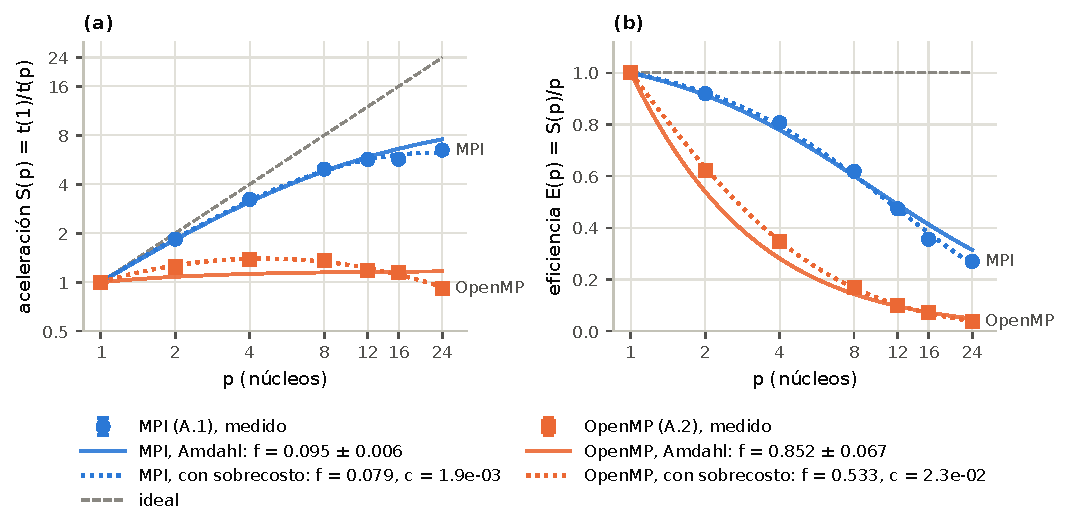
\includegraphics[width=0.97\textwidth]{figuras/A3_escalamiento.pdf}
\caption{(a) Aceleración y (b) eficiencia de MPI (A.1, SCF completo) y OpenMP (A.2, 4 iteraciones), con la
curva ideal, la ley de Amdahl ajustada (línea continua) y el modelo con sobrecosto (punteada). Barras de error:
desviación estándar de 3 repeticiones (menores que los símbolos).}
\label{fig:A3}
\end{figure}

\begin{table}[H]
\centering\small
\begin{adjustbox}{max width=\textwidth}\begin{tabular}{l rr r rrr rr}
\toprule
 & \multicolumn{3}{c}{Amdahl} & \multicolumn{3}{c}{con sobrecosto $c\,(p-1)$} & \multicolumn{2}{c}{Karp--Flatt $e(p)$} \\
\cmidrule(lr){2-4}\cmidrule(lr){5-7}\cmidrule(lr){8-9}
serie & $f$ & $\chi^2_\nu$ & $1/f$ & $f$ & $c$ & $p^{*}$ & $p=2$ & $p=24$ \\
\midrule
MPI, corrida & 0.095 $\pm$ 0.006 & 53 & 10.5 & 0.079 $\pm$ 0.006 & $1.9\times10^{-3}$ & 22.1 & 0.088 & 0.117 \\
OpenMP, corrida & 0.852 $\pm$ 0.067 & 189 & 1.2 & 0.533 $\pm$ 0.031 & $2.3\times10^{-2}$ & 4.6 & 0.612 & 1.095 \\
MPI, por iteración & 0.101 $\pm$ 0.006 & 24 & 9.9 & 0.080 $\pm$ 0.009 & $1.7\times10^{-3}$ & 23.3 & 0.095 & 0.112 \\
OpenMP, por iteración & 0.935 $\pm$ 0.106 & 508 & 1.1 & 0.498 $\pm$ 0.038 & $3.5\times10^{-2}$ & 3.8 & 0.608 & 1.371 \\
\bottomrule
\end{tabular}
\end{adjustbox}
\caption{Ajustes por mínimos cuadrados ponderados de $1/S-1/p=f(1-1/p)\,[+\,c\,(p-1)]$ para $p>1$;
$\chi^2_\nu$ es el $\chi^2$ reducido y $p^{*}=\sqrt{(1-f)/c}$, el $p$ de máxima aceleración del segundo
modelo. Karp--Flatt: $e(p)=(1/S-1/p)/(1-1/p)$, la fracción serial que daría cada punto por sí solo.}
\label{tab:A3}
\end{table}

\paragraph{MPI.} La aceleración crece hasta $S(24)=6.49\pm0.13$ ($E=0.27$). Amdahl ajusta
$f=0.095\pm0.006$ (techo $1/f=10.5$), pero con $\chi^2_\nu=53$: la ley no describe los datos. La razón está en
la fracción de Karp--Flatt (Tabla~\ref{tab:A3}): no es constante, sube de 0.08 ($p\le8$) a 0.12 ($p\ge16$),
es decir, el límite no es solo una parte serial fija sino un sobrecosto que crece con $p$. El modelo con
sobrecosto lineal reduce $\chi^2_\nu$ a 17 con $f=0.079$ y $c=1.9\times10^{-3}$. Las causas, en orden de
importancia según los datos:
\begin{itemize}[leftmargin=*]
\item \textbf{Comunicación y granularidad.} El 98\,\% de cada iteración es el eigensolver de Davidson
(\cod{EDDAV}), y ahí se pierde la eficiencia (de 90.6 a 14.3~s por iteración entre 1 y 24 procesos, una
aceleración de 6.3). Con \cod{KPAR = 1} los $p$ procesos se reparten las 144 bandas: con 24 procesos cada uno
tiene 6, los productos de matrices del subespacio son pequeños, y la ortogonalización y la rotación del
subespacio necesitan comunicación entre todos los procesos en cada iteración. Fuera del SCF (arranque, fuerzas
y escritura) se va un 11\,\% del tiempo con cualquier $p$.
\item \textbf{Ancho de banda de memoria.} La meseta entre 12 y 16 procesos ($S=5.68$ y 5.69), ambos con todos
los procesos en el socket~0, y el salto a 24 procesos, que ocupan 18 núcleos del socket~0 y 6 del socket~1
(con su propio controlador de memoria), indican que el socket~0 satura su ancho de banda. La B.1 lo confirma
de forma directa (Sec.~\ref{sec:b1}).
\item \textbf{Balance de carga.} No es el problema: 144 es divisible por todos los $p$ medidos, así que cada
proceso tiene el mismo número de bandas.
\item \textbf{Hyperthreading.} No se usó (un hilo de hardware por núcleo, verificado en cada corrida).
\end{itemize}

\paragraph{OpenMP.} La aceleración máxima es 1.39 con 4 hilos; con 12 o más hilos cada iteración es tan lenta
como con 1 hilo y con 24 es más lenta ($S_\text{iter}=0.74$). Con $e(p)$ entre 0.6 y 1.4, Amdahl no tiene
sentido ($\chi^2_\nu=189$); el modelo con sobrecosto describe la forma ($p^{*}=4.6$, $S_\text{máx}=1.40$,
como se midió). Tres causas: (i) en VASP los hilos de OpenMP reemplazan la paralelización de las FFT de
\cod{NCORE}~\cite{vasp-par} y la documentación pide compilar con \cod{fftlib} si no se usan las FFT de
MKL~\cite{vasp-omp}; este binario no la tiene, y con una malla FFT pequeña ($32\times32\times64$) hay poco
trabajo por hilo frente al costo de sincronizarlos; (ii) los hilos se sincronizan muy a menudo: con la espera pasiva
(\cod{OMP\_WAIT\_POLICY=PASSIVE}), en la que los hilos se duermen en lugar de girar mientras esperan, cada
iteración fue 50--67\,\% más lenta; (iii) con 24 hilos el proceso abarca los dos
sockets y el tiempo por iteración salta de 97 a 129~s (B.3). El diagnóstico de hyperthreading de la A.2
mostró además que 2 hilos de OpenMP por núcleo físico hacen el cálculo más lento que en serie.

% =============================================================================
\section{Escalamiento débil e híbrido (B.1--B.3)}

\subsection{B.1: escalamiento débil}\label{sec:b1}
El problema crece con $p$ a través de los k-points: $p$ procesos MPI con \cod{KPAR = p} y una malla con
exactamente $3p$ k-points irreducibles (contados con la simetría de la supercelda y comprobados contra el
\cod{NKPTS} de VASP), de modo que cada proceso calcula 3 k-points con las 144 bandas y no se comunica con nadie
dentro del eigensolver. Todas las corridas convergieron en 18 iteraciones.

\begin{table}[H]
\centering\small
\begin{adjustbox}{max width=\textwidth}\begin{tabular}{r l r r r r r r r}
\toprule
$p$ & malla & NKPTS & $t$ (s) & $E_w$ & s/iter. & EDDAV (s/iter.) & mem./proceso (GB) & mem. total (GB) \\
\midrule
1 & 3$\times$3$\times$1 & 3 & 164.5 $\pm$ 0.5 & 1.000 $\pm$ 0.005 & 8.03 & 7.63 & 0.18 & 0.18 \\
2 & 3$\times$3$\times$2 & 6 & 169.4 $\pm$ 0.5 & 0.971 $\pm$ 0.004 & 8.27 & 7.87 & 0.24 & 0.49 \\
4 & 5$\times$5$\times$3 & 12 & 180.0 $\pm$ 0.8 & 0.914 $\pm$ 0.005 & 8.74 & 8.33 & 0.38 & 1.51 \\
8 & 6$\times$6$\times$4 & 24 & 205.8 $\pm$ 0.3 & 0.799 $\pm$ 0.003 & 9.94 & 9.50 & 0.65 & 5.16 \\
12 & 10$\times$10$\times$3 & 36 & 235.8 $\pm$ 0.3 & 0.698 $\pm$ 0.003 & 11.34 & 10.82 & 0.91 & 10.95 \\
16 & 14$\times$14$\times$2 & 48 & 284.4 $\pm$ 0.7 & 0.578 $\pm$ 0.002 & 13.62 & 13.03 & 1.18 & 18.88 \\
24 & 10$\times$10$\times$6 & 72 & 327.3 $\pm$ 1.0 & 0.503 $\pm$ 0.002 & 15.42 & 14.78 & 1.72 & 41.33 \\
\bottomrule
\end{tabular}
\end{adjustbox}
\caption{Escalamiento débil: $E_w(p)=t(1)/t(p)$; s/iter.: tiempo medio por iteración SCF; EDDAV: el
eigensolver de Davidson (95\,\% de cada iteración). Memoria: VmHWM, máximo por proceso y suma de todos.}
\label{tab:B1}
\end{table}

\begin{figure}[H]
\centering
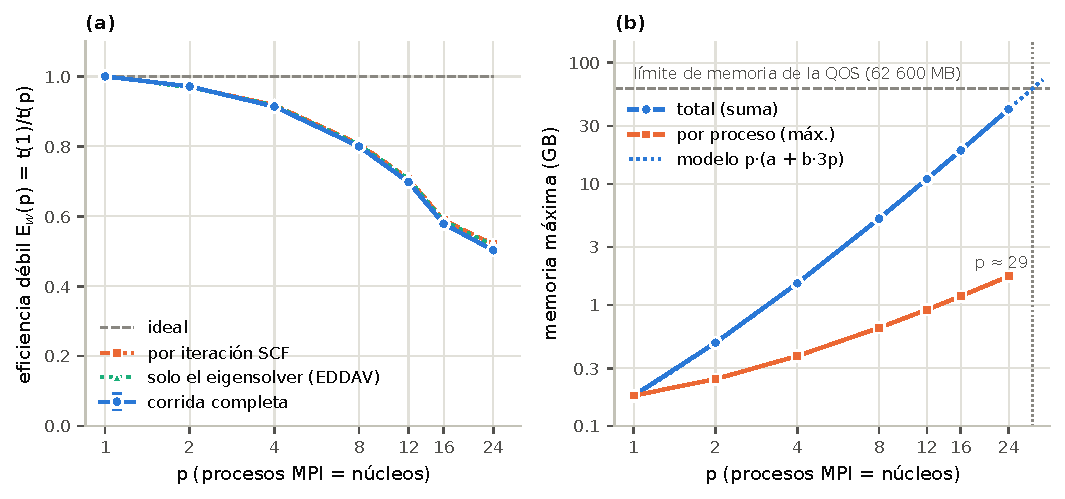
\includegraphics[width=0.97\textwidth]{figuras/B1_debil.pdf}
\caption{(a) Eficiencia débil de la corrida, por iteración y del eigensolver solo; las tres coinciden.
(b) Memoria máxima por proceso y total; la línea punteada es $p\,(a+b\cdot3p)$ con $a=112.5$~MB y
$b=22.9$~MB por k-point, ajustados a los datos.}
\label{fig:B1}
\end{figure}

$E_w$ baja a $0.50$ con 24 procesos (Tabla~\ref{tab:B1}, Fig.~\ref{fig:B1}a). Como el número de iteraciones
es el mismo, $E_w$ por iteración coincide, y como el eigensolver por sí solo pierde exactamente lo mismo
(7.6~s por iteración con 1 proceso, 14.8~s con 24), la pérdida no viene de la comunicación (las partes que
sí comunican, densidad y potencial, suman menos de 1~s) ni del número de iteraciones: cada proceso hace el
mismo trabajo, solo y más despacio, cuantos más procesos trabajan a la vez. Es contención por recursos
compartidos del nodo: los 6 canales de memoria y los 24.75~MB de L3 de cada socket se reparten entre más
procesos, y la frecuencia de turbo baja al activarse más núcleos~\cite{intel}.

\textbf{Problemas de memoria.} La memoria por proceso no es constante: crece de 0.18 a 1.72~GB porque, aunque
cada proceso solo calcula sus 3 k-points, VASP guarda en cada proceso las funciones de onda de \emph{todos}
los k-points~\cite{vasp-mem}. El OUTCAR lo confirma: con $p=24$ las funciones de onda ocupan 1525~MB en el
proceso 0, 24 veces más que con $p=1$, y el ajuste da 22.9~MB por k-point, lo que pesan las 144 bandas
$\times$ 8815 ondas planas en complejo doble (19.4~MB) más los proyectores. Con $\text{NKPTS}=3p$ la memoria
total crece como $p^2$: de 0.18~GB a 41.3~GB, y pasaría los 62\,600~MB de la QOS en $p\approx29$
(Fig.~\ref{fig:B1}b). Para un sistema mayor (más átomos) la memoria por k-point crece además como $N^2$
(bandas $\times$ ondas planas), así que el escalamiento débil por k-points con KPAR se queda sin memoria
antes que sin núcleos.

\subsection{B.2: paralelismo híbrido con 24 núcleos}
\begin{table}[H]
\centering\small
\begin{adjustbox}{max width=\textwidth}\begin{tabular}{c r r r r r r c}
\toprule
$N_\mathrm{MPI}\times N_\mathrm{OMP}$ & $n$ & $t$ (s) & s/iter. & $S=t(1)/t$ & mem./proceso (GB) & mem. total (GB) & 2 sockets \\
\midrule
24$\times$1 & 3 & 89.3 $\pm$ 1.3 & 14.3 & 6.62 $\pm$ 0.11 & 0.17 & 3.95 & 0 de 24 \\
12$\times$2 & 3 & 92.0 $\pm$ 0.8 & 14.6 & 6.42 $\pm$ 0.08 & 0.20 & 2.36 & 0 de 12 \\
8$\times$3 & 3 & 107.1 $\pm$ 0.4 & 17.1 & 5.51 $\pm$ 0.05 & 0.23 & 1.84 & 0 de 8 \\
6$\times$4 & 3 & 123.9 $\pm$ 0.9 & 20.6 & 4.77 $\pm$ 0.05 & 0.27 & 1.62 & 1 de 6 \\
4$\times$6 & 3 & 152.5 $\pm$ 1.6 & 25.8 & 3.87 $\pm$ 0.05 & 0.34 & 1.35 & 0 de 4 \\
2$\times$12 & 3 & 311.0 $\pm$ 1.7 & 58.4 & 1.90 $\pm$ 0.02 & 0.56 & 1.11 & 1 de 2 \\
1$\times$24 & 4 & 644.6 $\pm$ 2.2 & 129.5 & 0.92 $\pm$ 0.01 & 1.00 & 1.00 & 1 de 1 \\
\bottomrule
\end{tabular}
\end{adjustbox}
\caption{Híbrido $N_\text{MPI}\times N_\text{OMP}=24$, carga de 4 iteraciones; $t(1)=590.8\pm5.1$~s es la
$p=1$ de la A.2 con la misma carga. $1\times24$ suma las 3 corridas de la A.2 y una nueva. Última columna:
procesos cuya máscara incluye núcleos de los dos sockets.}
\label{tab:B2}
\end{table}

\begin{figure}[H]
\centering
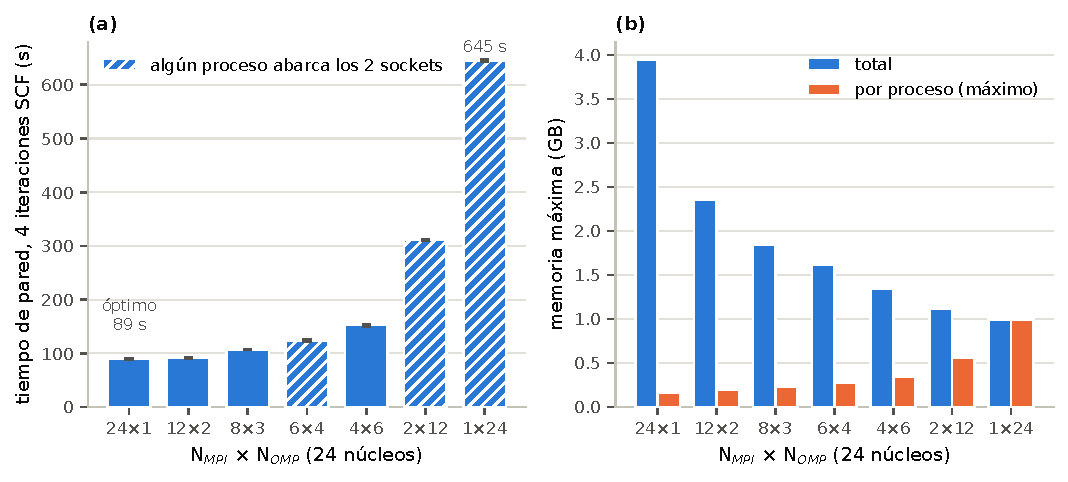
\includegraphics[width=0.97\textwidth]{figuras/B2_hibrido.pdf}
\caption{(a) Tiempo por combinación (rayado: algún proceso abarca los dos sockets). (b) Memoria máxima total
y por proceso.}
\label{fig:B2}
\end{figure}

\textbf{Afinidad.} En las 22 corridas la máscara real de cada proceso tuvo exactamente $N_\text{OMP}$ núcleos
físicos con un hilo de hardware cada uno, sin núcleos compartidos (\cod{afinidad.txt}), y el monitor vio los
hilos de VASP en $N_\text{MPI}\times N_\text{OMP}=24$ núcleos distintos, con \cod{OMP\_PLACES=cores} y
\cod{OMP\_PROC\_BIND=close}. El paso de \cod{srun} usó \cod{--hint=nomultithread}, que Slurm no permite
combinar con \cod{--cpu-bind=cores}; la máscara resultante ya restringe cada tarea a sus núcleos, como se
verificó en cada corrida.

\textbf{Óptimo.} El más rápido es MPI puro, $24\times1$ ($89.3\pm1.3$~s). El tiempo crece de forma monótona
con el número de hilos: cada hilo de más reemplaza a un proceso MPI que paralelizaba bien (bandas) por un hilo
que paraleliza mal (FFT pequeñas sin \cod{fftlib}). Pero $12\times2$ queda a solo 3\,\% ($92.0\pm0.8$~s) con
40\,\% menos memoria (2.36 frente a 3.95~GB), porque cada proceso MPI replica las mallas, los proyectores y los
búferes, mientras que los hilos de un proceso comparten una sola copia: la memoria total baja de 3.95~GB con
24 procesos a 1.00~GB con 1. Para un sistema que no cabe en memoria, $12\times2$ es la opción.

\subsection{B.3: topología y NUMA}
Cada socket tiene su propio controlador de memoria (6 canales) y su propia caché L3~\cite{intel}: es un nodo
NUMA, en el que un núcleo accede más rápido a la memoria de su socket que a la del otro, a través del enlace
entre sockets. Linux coloca cada página en el socket del hilo que la toca primero, de modo que un proceso que
abarca los dos sockets tiene parte de sus hilos trabajando sobre memoria remota, con más latencia y menos ancho
de banda, y sus barreras y su tráfico de coherencia de caché cruzan el enlace. En los datos: (i) con OpenMP,
pasar de 16 hilos (todos en un mismo socket) a 24 (18 + 6) sube cada iteración de 97 a 129~s (+33\,\%), mucho
más que el paso de 12 a 16 hilos (+3\,\%); (ii) con MPI puro, donde cada proceso usa solo su memoria local, sumar el
segundo socket \emph{ayuda} (de $S=5.69$ con 16 procesos a 6.49 con 24), porque aporta ancho de banda;
(iii) en la B.2 los 24 núcleos asignados fueron siempre 18 del socket~0 y 6 del socket~1, así que con
$4\times6$ cada proceso cabe en un socket y con $6\times4$ uno de los seis queda partido. Por eso el óptimo
híbrido depende de la topología: las combinaciones naturales son las que dejan cada proceso dentro de un socket
(y de su banco de memoria), y con 24 núcleos repartidos 18 + 6 la combinación con $N_\text{OMP}$ divisor de 6
evita los procesos partidos. Con un nodo completo, la opción híbrida natural sería 2 procesos $\times$ 18 hilos,
uno por socket, o más procesos por socket.

% =============================================================================
\section{Precisión numérica y reproducibilidad (C.1--C.2)}

\subsection{C.1: reproducibilidad con $p$}\label{sec:c1}
Se comparó la energía total convergida del caso base con $p$ procesos MPI (A.1). La fuente es la última línea
\cod{DAV} del OSZICAR, con 12 cifras significativas: su resolución es $10^{-9}$~eV
$=2.7\times10^{4}\,\eps|E|$, con $\eps=2^{-52}=2.22\times10^{-16}$ y $|E|=166.1$~eV.

\begin{table}[H]
\centering\small
\begin{adjustbox}{max width=\textwidth}\begin{tabular}{r c l r r r}
\toprule
$p$ & valores distintos en 3 rep. & $E(p)$ (eV, OSZICAR) & $E(p)-E(1)$ (eV) & $|\Delta E|/|E(1)|$ & $|\Delta E|/(\varepsilon_\mathrm{mach}|E(1)|)$ \\
\midrule
1 & 1 & -166.103007467 & 0 & 0 & 0 \\
2 & 1 & -166.103007469 & $-2.0\times10^{-9}$ & $1.2\times10^{-11}$ & $5.4\times10^{4}$ \\
4 & 1 & -166.103007470 & $-3.0\times10^{-9}$ & $1.8\times10^{-11}$ & $8.1\times10^{4}$ \\
8 & 1 & -166.103007471 & $-4.0\times10^{-9}$ & $2.4\times10^{-11}$ & $1.1\times10^{5}$ \\
12 & 1 & -166.103007478 & $-1.1\times10^{-8}$ & $6.6\times10^{-11}$ & $3.0\times10^{5}$ \\
16 & 1 & -166.103007478 & $-1.1\times10^{-8}$ & $6.6\times10^{-11}$ & $3.0\times10^{5}$ \\
24 & 1 & -166.103007493 & $-2.6\times10^{-8}$ & $1.6\times10^{-10}$ & $7.0\times10^{5}$ \\
\bottomrule
\end{tabular}
\end{adjustbox}
\caption{Energía total convergida con $p$ procesos MPI (3 repeticiones por $p$; las tres dieron el mismo
número en todos los casos). Pedido por el enunciado: $p=1,4,16,24$; se agregan los demás.}
\label{tab:C1}
\end{table}

\begin{table}[H]
\centering\small
\begin{adjustbox}{max width=\textwidth}\begin{tabular}{r l r l r}
\toprule
$N_\mathrm{MPI}$ & $N_\mathrm{OMP}$ medidos & corridas & $E$ tras 4 iteraciones (eV) & $E - E(1\times1)$ (eV) \\
\midrule
1 & 1, 2, 4, 8, 12, 16, 24 & 25 & -173.683422006 & 0 \\
2 & 1, 12 & 6 & -173.683422010 & $-4.0\times10^{-9}$ \\
4 & 1, 6 & 6 & -173.683422011 & $-5.0\times10^{-9}$ \\
6 & 4 & 3 & -173.696097605 & $-1.3\times10^{-2}$ \\
8 & 1, 3 & 6 & -173.683422012 / -173.683422013 & $-6.0\times10^{-9}$ \\
12 & 1, 2 & 6 & -173.696097606 & $-1.3\times10^{-2}$ \\
16 & 1 & 3 & -173.704100338 & $-2.1\times10^{-2}$ \\
24 & 1 & 6 & -173.715733479 & $-3.2\times10^{-2}$ \\
\bottomrule
\end{tabular}
\end{adjustbox}
\caption{Energía después de exactamente 4 iteraciones (pasos sin autoconsistencia y sin criterio de parada)
con $N_\mathrm{MPI}$ procesos y $N_\mathrm{OMP}$ hilos, de todas las corridas de la A.1, la A.2 y la B.2:
depende solo del número de procesos MPI.}
\label{tab:C1b}
\end{table}

\begin{table}[H]
\centering\small
\begin{tabular}{l r r r}
\toprule
precisión & $p$ & diferencia con $p=1$ ($\varepsilon_\mathrm{mach}$) & error frente a la suma exacta ($\varepsilon_\mathrm{mach}$) \\
\midrule
doble (\texttt{float64}) & 1 & 0 & 24 \\
doble (\texttt{float64}) & 4 & 19 & 5 \\
doble (\texttt{float64}) & 16 & 23 & 1 \\
doble (\texttt{float64}) & 24 & 20 & 4 \\
simple (\texttt{float32}) & 1 & 0 & 88 \\
simple (\texttt{float32}) & 4 & 93 & 5 \\
simple (\texttt{float32}) & 16 & 84 & 4 \\
simple (\texttt{float32}) & 24 & 83 & 5 \\
\bottomrule
\end{tabular}

\caption{Suma de $2^{20}$ números uniformes en $[0,1)$ repartida en $p$ bloques, como una reducción con $p$
procesos (suma secuencial en cada bloque y luego de las sumas parciales), en precisión doble y simple, en
unidades del $\eps$ de cada una (\cod{analisis/parteC\_analisis.py}, semilla fija).}
\label{tab:C1c}
\end{table}

\textbf{Resultado.} Para un mismo $p$, las 3 repeticiones dan el mismo número (12 cifras). Entre distintos $p$,
la energía difiere de la de $p=1$ en $2\times10^{-9}$ a $2.6\times10^{-8}$~eV, creciendo con $p$: de
$5\times10^{4}$ a $7\times10^{5}\,\eps|E|$ (Tabla~\ref{tab:C1}). Esto es, a la vez, mucho más que el error de
redondeo de una sola reducción y muchísimo menos de lo que importa en física.

\textbf{Relación con el orden de las reducciones.} La suma en punto flotante no es asociativa: al cambiar $p$
cambia el orden en que \cod{MPI\_Allreduce} junta las sumas parciales (densidad, energías, productos escalares
entre bandas repartidas). La Tabla~\ref{tab:C1c} muestra el tamaño del efecto en una sola suma: cambiar
el número de bloques mueve el resultado unas 20~$\eps$ en doble precisión (y unas 90 en simple). En VASP ese
redondeo distinto ocurre en miles de reducciones por iteración, y el SCF es un proceso iterativo no lineal que
propaga las perturbaciones; el resultado final solo queda fijado dentro del criterio de convergencia:
\cod{EDIFF}~$=10^{-6}$~eV~$=2.7\times10^{7}\,\eps|E|$, que es 40 a 500 veces mayor que las diferencias
observadas. Las diferencias medidas son, entonces, la huella del orden de las reducciones amplificada por el
SCF y acotada por la tolerancia; son seis órdenes de magnitud menores que 1~meV, de modo que todos los $p$ dan
la misma física.

\textbf{Qué cambia el resultado y qué no.} Antes de converger (Tabla~\ref{tab:C1b}) se ve con claridad la
fuente: los hilos de OpenMP no cambian ni la última cifra (de 1 a 24 hilos, la misma energía), pero
el número de procesos MPI sí. Con $N\le8$ procesos las diferencias son de $6\times10^{-9}$~eV (redondeo), y con
6, 12, 16 y 24 la energía después de 4 iteraciones cambia hasta 32~meV: al repartir las bandas entre más
procesos, el algoritmo de Davidson por bloques procesa las bandas en otros grupos y sigue otro camino hacia la
misma solución. Después de converger, todos coinciden en $2.6\times10^{-8}$~eV. Por eso la reproducibilidad
se compara siempre con resultados convergidos. Además se observó una variación de la última cifra
($10^{-9}$~eV) entre repeticiones idénticas en algunas corridas con KPAR, en una combinación híbrida y en 2 de
10 ENCUT con $p=1$: no depende de $p$, sino de alguna elección en tiempo de ejecución; una causa conocida es la
planificación de FFTW por medición de tiempos, que no es reproducible bit a bit~\cite{fftw-rep} (no verifiqué
qué modo usa este binario).

\subsection{C.2: precisión frente a costo}\label{sec:c2}
Se varió ENCUT de 250 a 800~eV con la malla $3\times3\times1$ (3 k-points) en 1 núcleo, SCF completo y 3
repeticiones (una serie por job, en orden ascendente, descendente y mezclado). El error de truncamiento de la
base por átomo casi no depende de la malla, y con 3 k-points la serie costó 2.4~h-núcleo en lugar de unas 30.
El error es $|E(\text{ENCUT})-E(800\,\text{eV})|/23$.

\begin{figure}[H]
\centering
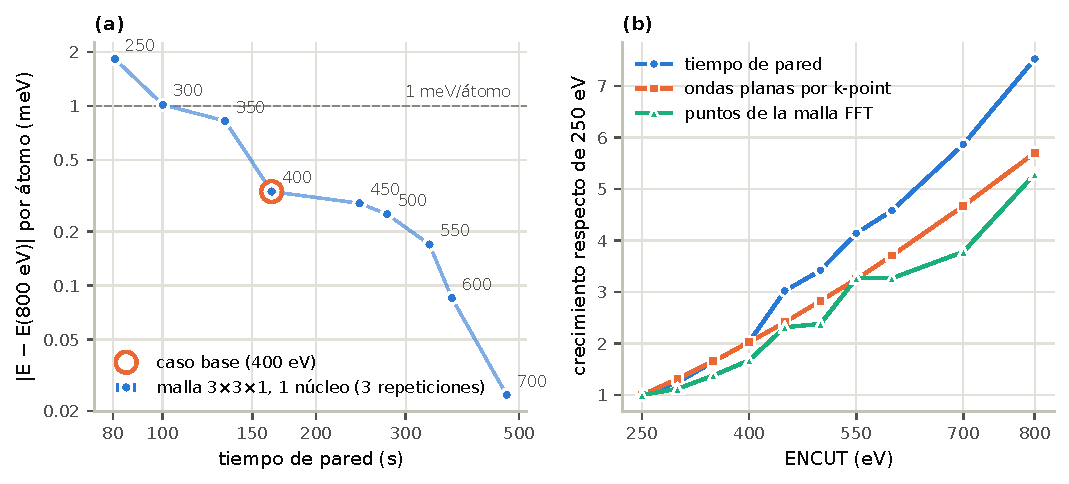
\includegraphics[width=0.97\textwidth]{figuras/C2_precision_costo.pdf}
\caption{(a) Error por átomo frente al tiempo de pared (barras horizontales: desviación estándar de 3
repeticiones); los números son el ENCUT en eV. (b) Crecimiento del tiempo, de las ondas planas por k-point y de
los puntos de la malla FFT respecto de 250~eV.}
\label{fig:C2}
\end{figure}

\begin{table}[H]
\centering\small
\begin{adjustbox}{max width=\textwidth}\begin{tabular}{r r r r l r r}
\toprule
ENCUT (eV) & $t$ (s) & $t/t(400)$ & ondas planas & malla FFT & mem. (MB) & error (meV/átomo) \\
\midrule
250 & 80.7 $\pm$ 0.3 & 0.49 & 4359 & 28$\times$28$\times$50 & 115 & 1.828 \\
300 & 100.2 $\pm$ 0.1 & 0.61 & 5725 & 28$\times$28$\times$56 & 133 & 1.016 \\
350 & 132.8 $\pm$ 0.4 & 0.81 & 7218 & 30$\times$30$\times$60 & 157 & 0.826 \\
400 & 163.8 $\pm$ 0.5 & 1.00 & 8815 & 32$\times$32$\times$64 & 184 & 0.334 \\
450 & 243.6 $\pm$ 2.4 & 1.49 & 10509 & 36$\times$36$\times$70 & 227 & 0.287 \\
500 & 275.9 $\pm$ 0.2 & 1.68 & 12324 & 36$\times$36$\times$72 & 245 & 0.250 \\
550 & 334.0 $\pm$ 0.8 & 2.04 & 14161 & 40$\times$40$\times$80 & 298 & 0.169 \\
600 & 369.4 $\pm$ 1.4 & 2.26 & 16155 & 40$\times$40$\times$80 & 316 & 0.085 \\
700 & 473.2 $\pm$ 0.8 & 2.89 & 20358 & 42$\times$42$\times$84 & 375 & 0.025 \\
800 & 607.0 $\pm$ 0.9 & 3.71 & 24849 & 48$\times$48$\times$90 & 477 & referencia \\
\bottomrule
\end{tabular}
\end{adjustbox}
\caption{Serie de ENCUT (18 iteraciones SCF en todos los casos).}
\label{tab:C2}
\end{table}

\textbf{Punto de rendimientos decrecientes: 400~eV.} De 250 a 400~eV el error baja 5.5 veces (de 1.83 a
0.33~meV/átomo) a cambio del doble de tiempo; de 400 a 500~eV casi no baja (0.33 → 0.25) aunque el tiempo
sube 68\,\%, y el primer paso, de 400 a 450~eV, cuesta un 49\,\% más por solo un 14\,\% menos de error
(Fig.~\ref{fig:C2}a). La Fig.~\ref{fig:C2}b explica el salto: el tiempo no sigue solo al número de ondas planas
(que crece como $\text{ENCUT}^{3/2}$) sino a la malla FFT, que crece a saltos y en 450~eV pasa de
$32\times32\times64$ a $36\times36\times70$, con un factor 7 menos eficiente para la FFT. Con 400~eV el error
ya está bajo 1~meV/átomo, la precisión habitual para energías de formación de defectos, y las diferencias de
energía convergen más rápido que las energías totales por cancelación de errores. Para comparar, la malla de
k-points del caso base ($10\times10\times3$) difiere en 0.0004~meV/átomo de una $10\times10\times6$ (B.1) y una
$6\times6\times3$ ya estaría en 0.002~meV/átomo con la mitad del tiempo: en el caso base, el error dominante es
el de ENCUT.

\textbf{Precisión simple frente a doble.} VASP~6.3.0 para CPU solo calcula en doble precisión, así que no se
pudo comparar con corridas. La tabla de la reducción da la escala: en simple, $\eps=2^{-23}=1.19\times10^{-7}$
y una sola suma de $10^6$ términos ya difiere en $\sim10^{-5}$ relativo según el orden. Para $|E|=166$~eV,
$\eps|E|=2\times10^{-5}$~eV en simple: el criterio \cod{EDIFF}~$=10^{-6}$~eV sería inalcanzable, porque pide
una precisión relativa de $6\times10^{-9}$, menor que el $\eps$ de la precisión simple.

% =============================================================================
\section{Recomendación (D.1)}

\begin{table}[H]
\centering\small
\begin{tabular}{l r r r}
\toprule
configuración (SCF completo del caso base) & núcleos & $t$ (min) & h-núcleo por cálculo \\
\midrule
1 proceso MPI, KPAR = 1 & 1 & 31.2 & 0.52 \\
2 procesos MPI, KPAR = 1 & 2 & 17.0 & 0.56 \\
4 procesos MPI, KPAR = 1 & 4 & 9.7 & 0.64 \\
8 procesos MPI, KPAR = 1 & 8 & 6.3 & 0.84 \\
12 procesos MPI, KPAR = 1 & 12 & 5.5 & 1.10 \\
16 procesos MPI, KPAR = 1 & 16 & 5.5 & 1.46 \\
24 procesos MPI, KPAR = 1 & 24 & 4.8 & 1.92 \\
12 procesos MPI, KPAR = 12 (B.1) & 12 & 3.9 & 0.79 \\
\bottomrule
\end{tabular}
\\[8pt]
\begin{tabular}{l r r}
\toprule
parte & jobs & h-núcleo \\
\midrule
Tarea 0: calibración final (K1--K7) & 7 & 2.00 \\
A.1: escalamiento fuerte MPI & 21 & 21.59 \\
A.2: diagnóstico de OpenMP (2 rondas) & 18 & 33.95 \\
A.2: barrido OpenMP (4 iteraciones) & 21 & 30.94 \\
B.1: escalamiento débil & 21 & 15.55 \\
B.2: híbrido MPI $\times$ OpenMP & 19 & 23.04 \\
C.2: serie de ENCUT & 3 & 2.37 \\
Pruebas e intentos previos (17--18 nov.) & 56 & 19.09 \\
\midrule
\textbf{total (de 250)} & 166 & \textbf{148.53} \\
\bottomrule
\end{tabular}

\caption{Arriba: costo de un cálculo SCF del caso base (h-núcleo $=p\,t$). Abajo: consumo del examen según
\cod{sacct} (CPUTimeRAW, \cod{phys\_fast}): los 166 jobs con JobID $\geq 528789$, desde el 17 de noviembre. El
registro del enunciado incluye además jobs anteriores que no son del examen (final de la Sec.~\ref{sec:d2}).}
\label{tab:D}
\end{table}

\noindent\textit{Para: compañeros del grupo de Física Aplicada que calculan defectos en WSe$_2$ con VASP en
Granado. Asunto: cómo correr un SCF de una supercelda de unos 20--30 átomos.}

\begin{enumerate}[leftmargin=*]
\item \textbf{Partición:} \cod{phys\_fast}. Un SCF de este tamaño tarda de 4 a 31~minutos, muy por debajo del
límite de 5~h. En mis 143 jobs del examen (17 a 22 de noviembre), el 98\,\% empezó menos de 1~minuto después de quedar
elegible y la espera máxima fue de 12.7~min (mediana: 0~s). Esa fue una semana tranquila; con la cola
congestionada la espera puede ser mucho mayor, así que conviene enviar pronto.
\item \textbf{Solo MPI, nada de OpenMP:} \cod{OMP\_NUM\_THREADS=1}, un proceso por núcleo físico, nunca 2 por
núcleo. Con este binario (sin \cod{fftlib}) OpenMP casi no acelera (máximo 1.39 con 4 hilos) y con 24 hilos es
más lento que en serie.
\item \textbf{Usen KPAR, no reparto de bandas:} con \cod{KPAR = 12} y 12 procesos el caso base tarda 3.9~min y
cuesta 0.79~h-núcleo; con 24 procesos y \cod{KPAR = 1}, 4.8~min y 1.92~h-núcleo. Es decir, la mitad de núcleos
da el resultado antes y 2.4 veces más barato, como recomienda VASP para celdas pequeñas con muchos
k-points~\cite{vasp-opt}. KPAR debe dividir al número de procesos y conviene que divida al número de k-points.
\cod{NCORE = 1}.
\item \textbf{Memoria:} con KPAR cada proceso guarda todos los k-points (0.9~GB por proceso aquí, 11~GB en
total con 12 procesos): pidan \cod{--mem=16G}, y para sistemas mayores revisen la memoria que estima el OUTCAR
antes de subir KPAR.
\item \textbf{Si hay muchos cálculos} (por ejemplo, varias posiciones del defecto), conviene correr varios jobs
pequeños a la vez en lugar de uno grande: con 4 procesos la eficiencia es 0.81 (0.64~h-núcleo por cálculo) y
con 24 es 0.27.
\item \textbf{Parámetros físicos:} ENCUT~$=400$~eV (0.33~meV/átomo); la malla $10\times10\times3$ está más que
convergida, y una $6\times6\times3$ basta para la energía total (verifiquen la convergencia de la energía de
formación).
\end{enumerate}

\noindent Plantilla mínima (revisen la afinidad con \cod{--cpu-bind=verbose} en el archivo de salida; con
\cod{mpirun}, OpenMPI ignora la asignación de Slurm y ata todos los procesos al núcleo~0):
{\small
\begin{verbatim}
#!/bin/bash
#SBATCH --partition=phys_fast
#SBATCH --nodes=1
#SBATCH --ntasks=12
#SBATCH --cpus-per-task=1
#SBATCH --hint=nomultithread
#SBATCH --mem=16G
#SBATCH --time=01:00:00
module load vasp/6.3.0-gnu9-openmp
export LD_LIBRARY_PATH=$HOME/lib:$LD_LIBRARY_PATH # libfftw3*.so.3 copiadas del login
export OMP_NUM_THREADS=1                          # INCAR: KPAR = 12, NCORE = 1
srun --mpi=pmix --cpu-bind=verbose,cores vasp_std
\end{verbatim}}

% =============================================================================
\section{Discusión: limitaciones y sistemas mayores (D.2)}\label{sec:d2}

\textbf{Limitaciones.} (i) \emph{Un sistema pequeño}: 23 átomos y 144 bandas; con pocas bandas por proceso
la comunicación pesa pronto, y las conclusiones sobre MPI y OpenMP cambian con el tamaño. (ii) \emph{Un solo
nodo}: todas las mediciones fueron en \cod{granado-compute-14}; eso controla la variable ``nodo'', pero no mide
la variabilidad entre nodos. (iii) \emph{Pocas repeticiones}: 3 por punto; la dispersión fue pequeña
(${\le}2$\,\%), pero todas se midieron en dos noches con la cola casi vacía y sin carga ajena; con el clúster
cargado los tiempos y la cola empeoran. (iv) \emph{Cargas cortas}: la A.2 y la B.2 usan 4 iteraciones; el tiempo
de un SCF completo se infiere por iteración. (v) \emph{Asignación no controlada}: los 24 núcleos quedaron
repartidos 18 + 6 entre sockets (Slurm llena primero el socket~0), lo que afecta la B.3. (vi) \emph{Un binario}:
las conclusiones sobre OpenMP valen para VASP sin \cod{fftlib}. (vii) La memoria total es la suma de los
VmHWM, que cuenta dos veces las páginas compartidas.

\textbf{Un sistema 10 veces mayor que no cabe en un nodo} (unos 230 átomos): las funciones de onda por
k-point crecen como $N^2$ (100 veces: unos 2~GB por k-point) y el costo como $N^2$--$N^3$, aunque la zona de
Brillouin más pequeña pide unas 10 veces menos k-points. Las conclusiones cambiarían así:
(i) \cod{KPAR} dejaría de ser la primera opción, porque cada proceso guarda todos los k-points; se usaría
solo entre nodos, con 1 a 4 k-points por grupo. (ii) Dentro de cada nodo habría que repartir las bandas y,
sobre todo, las FFT (\cod{NCORE} $>1$, del orden de los núcleos de un socket), para que la comunicación más
intensa quede dentro del socket y no cruce la red. (iii) OpenMP volvería a ser útil: la B.2 muestra que pasar de
$24\times1$ a $12\times2$ cuesta 3\,\% de tiempo y ahorra 40\,\% de memoria, y cuando la memoria es el límite
eso decide; con más trabajo por FFT, además, los hilos rendirían mejor (sobre todo con \cod{fftlib}).
(iv) La eficiencia de MPI mejoraría (Gustafson: más trabajo por proceso). (v) Con las reglas del examen no se
podría correr: la QOS limita cada job a 24 CPUs y 62\,600~MB, y \cod{phys\_fast} a 5~h; haría falta una QOS
de varios nodos y \cod{phys\_general} (1 día) con reinicios.

% =============================================================================
\section{Conclusiones}
\begin{itemize}[leftmargin=*]
\item MPI escala de forma moderada ($S(24)=6.5$) y está limitado por un sobrecosto que crece con $p$
(comunicación del reparto de bandas y ancho de banda de memoria), no por una fracción serial fija.
\item OpenMP no sirve con este binario: $S\le1.39$, y con un proceso que abarca dos sockets empeora.
\item En escalamiento débil, la pérdida de eficiencia ($E_w(24)=0.50$) es contención de recursos del nodo y no
comunicación; la memoria crece como $p^2$ con KPAR y es el primer límite.
\item El óptimo híbrido con 24 núcleos es MPI puro; $12\times2$ es la alternativa cuando falta memoria.
\item Los resultados no dependen de $p$ más allá de $2.6\times10^{-8}$~eV, muy por debajo de la tolerancia
del SCF; ENCUT~$=400$~eV es el punto de rendimientos decrecientes.
\item Para el grupo: \cod{phys\_fast}, MPI puro, \cod{KPAR = 12} en 12 núcleos: 3.9~min y 0.79~h-núcleo.
\end{itemize}

\paragraph{Reproducibilidad y consumo.} El repositorio contiene las entradas (sin el POTCAR, por licencia),
todos los scripts de Slurm, los datos crudos y la evidencia de cada corrida, y los scripts de \cod{analisis/}
que generan cada figura y cada tabla de este reporte; el \cod{README.md} explica cómo reproducir todo. El
consumo del examen, según \cod{sacct}, fue de 148.5 de 250~h-núcleo en 166 jobs (JobID $\geq 528789$,
Tabla~\ref{tab:D}). El registro que pide el enunciado (\cod{datos/sacct\_registro\_examen.txt}) empieza el 7 de
septiembre y por eso incluye también 370 jobs de investigación anteriores al examen, con mi misma cuenta
(11\,683~h-núcleo), que no usan su presupuesto; \cod{datos/sacct\_registro\_LEEME.md} explica la separación.

\begin{thebibliography}{9}\small
\bibitem{intel} Intel. \emph{Intel Xeon Gold 6140 Processor (24.75M Cache, 2.30 GHz): especificaciones}.
\url{https://www.intel.com/content/www/us/en/products/sku/120485.html}
\bibitem{vasp-par} VASP Wiki. \emph{Category: Parallelization}. \url{https://vasp.at/wiki/Parallelization}
\bibitem{vasp-omp} VASP Wiki. \emph{Combining MPI and OpenMP}. \url{https://vasp.at/wiki/Combining_MPI_and_OpenMP}
\bibitem{vasp-mem} VASP Wiki. \emph{Memory requirements}. \url{https://vasp.at/wiki/Memory_requirements}
\bibitem{vasp-opt} VASP Wiki. \emph{Optimizing the parallelization}. \url{https://vasp.at/wiki/Optimizing_the_parallelization}
\bibitem{fftw-rep} F. Locher \emph{et al.} \emph{TIFF: gyrofluid turbulence in full-f and full-k}, sec.~V
(reproducibilidad con FFTW). arXiv:2306.02354.
\bibitem{amdahl} G. M. Amdahl, AFIPS Conf. Proc. \textbf{30}, 483 (1967); J. L. Gustafson, Commun. ACM
\textbf{31}, 532 (1988); A. H. Karp y H. P. Flatt, Commun. ACM \textbf{33}, 539 (1990).
\end{thebibliography}

\end{document}
